% Chapter 1

\chapter{Introduction} % Main chapter title

\label{Chapter1} % For referencing the chapter elsewhere, use \ref{Chapter1} 

\lhead{Chapter 1. \emph{Introduction}} % This is for the header on each page - perhaps a shortened title

%----------------------------------------------------------------------------------------

Many-Task Computing (MTC)\cite{mtc} is a new computing paradigm that attempts to place itself in-between High-Throughput Computing (HTC) and High-Performance Computing (HPC). The core idea of MTC is that it uses large amounts of computing resources over short periods of time, in order to complete multiple tasks. While a common metric in HTC is the number of tasks fulfilled per month, MTC is usually quantified in tasks per second. Also, as opposed to other paradigms that use message passing as a way to communicate between successive steps in a computation, MTC couples its compute phases via files. Because of this, another common metric of MTC is megabytes per second (MB/s).

Any computing task that is comprised of multiple small parallel jobs is a good fit for MTC. Multiple applications have been found good fits for MTC\cite{mtc}, spanning domains like astronomy, astrophysics, economic modelling, pharmaceutics, chemistry, bioinformatics, neuroscience, data analytics, data mining and biometrics.

MTC exhibits a specific set of technical particularities which need to be properly supported in order to obtain good performance. The high number of parallel tasks that need to be executed underlines the importance of a streamlined scheduling system. Besides that, the way the tasks use files to communicate makes the overall performance largely dependant on the underlying filesystem performance. For the purpose of our subject, we will focus on the filesystem aspect.

Figure~\ref{fig:montage} shows an example workflow of Montage\cite{montage}, a software toolkit for astronomical image mosaicking. It shows the outline of a MTC workload, as well as the specific access patterns that emerge, such as data partitioning and aggregation.

\begin{figure}[H]
  \centering
    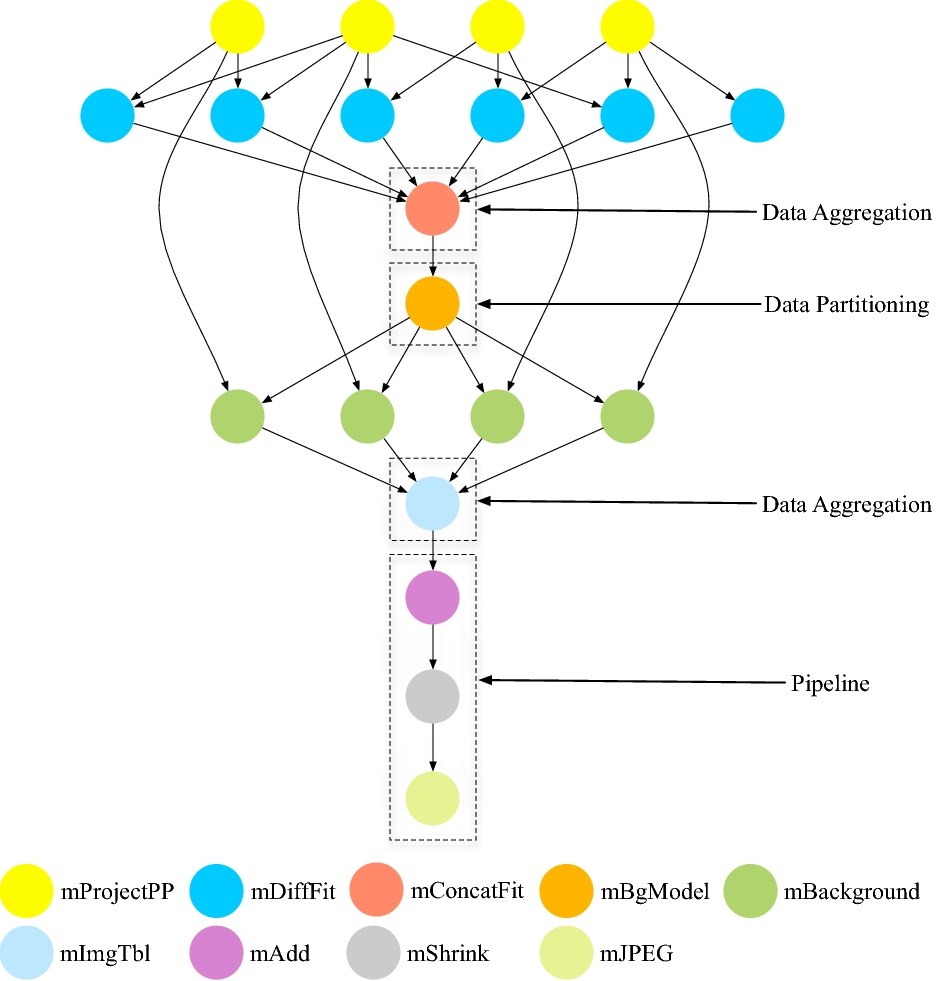
\includegraphics[scale=0.35]{Figures/montage.jpg}
    \rule{25em}{0.5pt}
  \caption[Montage workflow]{Montage workflow}
  \label{fig:montage}
\end{figure}

Typically, MTC jobs are run on clusters of compute nodes. These compute nodes need to share data files between them in order to complete the tasks that are assigned to them. Usually, files are locally stored on disk drives (either mechanical disk drives or solid state drives), and are sent over the network when a different node needs access. However, even with the fastest drives commercially available today, the transfer rates of disk drives are inferior to the bandwidth of InfiniBand connections that are used in clusters, considering the fact that a SATA link tops out at 3 GBps while InfiniBand 12X supports a 30 GBps data link. This shows that the bottleneck is not the network, but the storage technology. To overcome this bottleneck, RAM can be used as a storage medium. Obviously it cannot achieve the same storage capacity as regular disk drives, but that is not a problem for the purposes of MTC, as the data files used are not so large in size.

In order to make use of the high speed RAM and network connections that compute nodes in today's clusters have, research groups have started work on developing distributed, in-memory filesystems. These filesystems are specifically designed to support MTC workloads and yield better results than common network filesystems like NFS.

To illustrate how such filesystems work, we will describe two implementations - AMFS\cite{amfs} and MemFS\cite{memfs}.

\section{MemFS}

MemFS\cite{memfs} is a distributed, in-memory filesystem for MTC applications. Its motivating idea is that data locality is hard to preserve in MTC applications, and so a filesystem that is locality-agnostic could take advantage of the low-latency, high-bandwidth network connections that we have today and provide good performance for MTC applications. It has three main design goals:

\begin{enumerate}

\item maximize read and write throughput/bandwidth trying to achieve line-speed
\item achieve close-to-linear I/O operations scalability when increasing the number of compute nodes
\item reduce latency by storing data in memory and by improving the metadata protocol

\end{enumerate}

\begin{figure}[H]
  \centering
    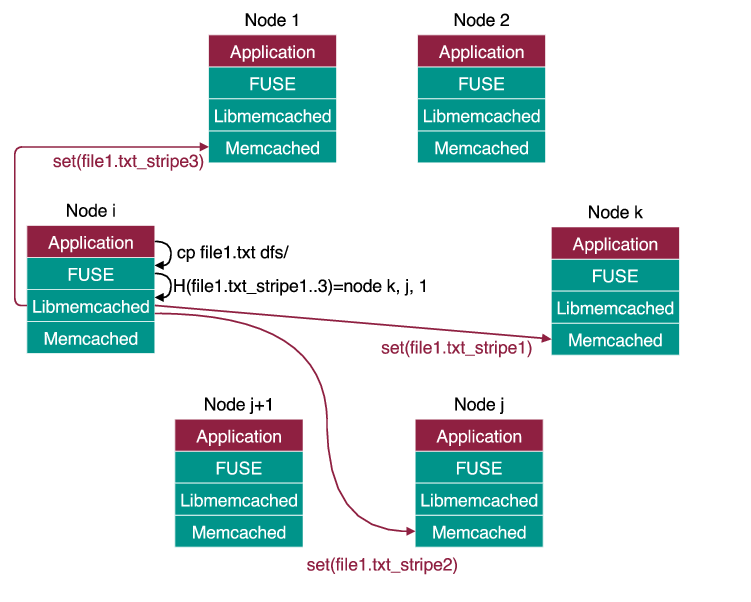
\includegraphics[scale=0.5]{Figures/memfs.png}
    \rule{25em}{0.5pt}
  \caption[MemFS design]{MemFS design}
  \label{fig:memfs}
\end{figure}

Its three main components are Memcached\cite{memcached}, a distributed cache system that is used in the industry, libmemcached\cite{libmemcached}, a client for interfacing with the Memcached server(s) and a FUSE\cite{fuse} filesystem that exposes the data storage mechanism to the MTC applications that run on top of MemFS.

% --------------

\section{AMFS}

AMFS\cite{amfs} is another distributed filesystem for MTC applications. In contrast to MemFS, it also includes an execution engine. This execution engine exposes a shell programming environment which application developers have to use to access distributed programming features, such as distributing the files in a folder across multiple nodes.

\begin{figure}[H]
  \centering
    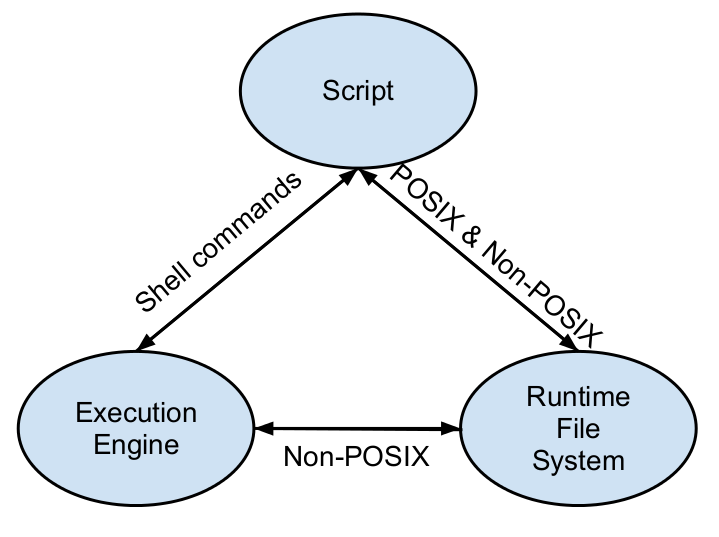
\includegraphics[scale=0.35]{Figures/amfs.png}
    \rule{25em}{0.5pt}
  \caption[AMFS design]{AMFS design}
  \label{fig:amfs}
\end{figure}

Another particularity of AMFS is that it tries to exploit data-locality. Its execution engine will try to run tasks on the nodes that already have the needed files, and only if this is not possible will it copy the needed files over to another node.

AMFS also stores file information in memory, but it decouples the medatada from the actual file blobs. Thus, it contains a metadata engine that keeps track of file properties and where the actual binary data is stored within the nodes.

% --------------


\section{Benchmarking MTC filesystems}

Besides the different storage medium (RAM), MTC-specific filesystems also target different access patterns. First, there is the usual 1-to-1 read pattern, where a node needs access to one file. In MTC workloads, it is probable that the file will reside on a different node's local storage. Second, there is the more complicated N-to-1 read pattern, where multiple nodes need to access the exact same file that is stored on a single node's local storage. In order for the MTC workload to achieve maximum performance, the underlying filesystem should make the most out of the network bandwidth, without creating bottlenecks because of contention.

In order to properly benchmark these filesystems, we need a tool that can simulate the MTC specific access patterns. This tool should be able to support a variable number of nodes, such that the scalability of the filesystem can be measured. Furthermore, the benchmark should be able to coordinate the nodes in a deterministic and synchronized manner in order to correctly reproduce access patterns such as N-to-1 reads. Finally, the results aggregation step should be built in, to facilitate tracking performance improvements between different test runs. Our solution provides all these features and, in addition, it uses a simple JSON\cite{json} file to specify complex test cases. We will detail all features later, in this study.


The rest of this study is structured as follows: Chapter 2 provides more context on benchmarking distributed MTC filesystems and related work. In Chapter 3 we discuss our implementation, as well as the design decisions we have made. Then, in Chapter 4 we evaluate the performance of our solution. Finally, Chapter 5 presents our conclusions.